\documentclass{beamer}
\setbeamertemplate{navigation symbols}{}

\usepackage{tikz}
\graphicspath{{..//src//images//}}

\setbeamercolor{frametitle}{fg=black,bg=white}
\setbeamercolor{title}{fg=black,bg=yellow!85!orange}
\usetheme{AnnArbor}

\beamersetuncovermixins{\opaqueness<1>{25}}{\opaqueness<2->{15}}
\begin{document}
\title{Clustering Overview}
\author{FRI}
\date{\today} 

\begin{frame}
\titlepage
\end{frame}

\begin{frame}
\frametitle{What is clustering?}
    \begin{itemize}
    \item partitioning into groups of similar objects
    \item hundreds of algorithms
    \end{itemize}

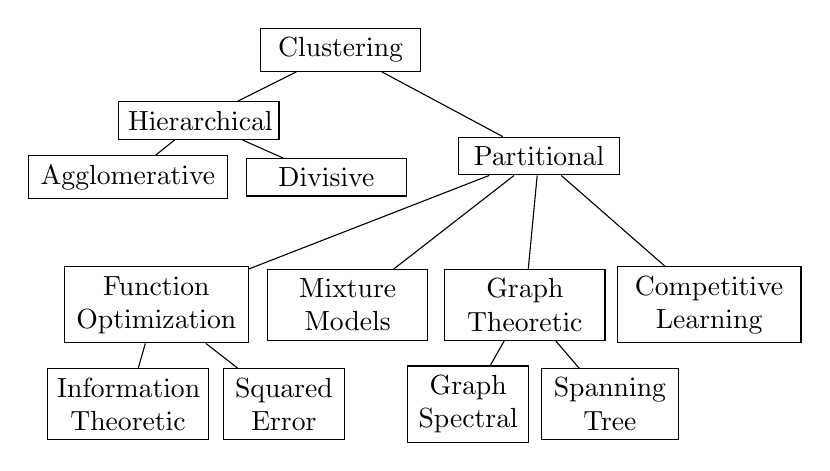
\begin{tikzpicture}[scale=0.9, text width=1.8cm, text centered]
    \tikzstyle{every node} = [rectangle,draw]

    \node (a) at (7, 5) {Clustering};
    \node (b) at (5, 4) {Hierarchical};
    \node (c) at (9.8, 3.5) {Partitional};

    \node (d) at (4, 3.2) [text width=2.3cm] {Agglomerative};
    \node (e) at (6.8, 3.2) {Divisive};

    \node (f) at (4.4, 1.4) [text width=2.1cm] {Function \\ Optimization};
    \node (g) at (7.1, 1.4) {Mixture \\ Models};
    \node (h) at (9.6, 1.4) {Graph \\ Theoretic};
    \node (i) at (12.2, 1.4) [text width=2.1cm] {Competitive \\ Learning};

    \node (j) at (4.0, 0.0) {Information \\ Theoretic};
    \node (k) at (6.2, 0.0) [text width=1.3cm] {Squared \\ Error};

    \node (l) at (8.8, 0.0) [text width=1.3cm] {Graph \\ Spectral};
    \node (m) at (10.8, 0.0) [text width=1.5cm] {Spanning \\ Tree};

    \draw [-] (a) -- (b);
    \draw [-] (a) -- (c);

    \draw [-] (b) -- (d);
    \draw [-] (b) -- (e);

    \draw [-] (c) -- (f);
    \draw [-] (c) -- (g);
    \draw [-] (c) -- (h);
    \draw [-] (c) -- (i);

    \draw [-] (f) -- (j);
    \draw [-] (f) -- (k);

    \draw [-] (h) -- (l);
    \draw [-] (h) -- (m);
\end{tikzpicture}
\end{frame}

\begin{frame}
\frametitle{k-means}
    \begin{itemize}
    \item well-known and widely used
    \item fast but produces equi-sized clusters (Voronoi)
    \item examples assigned to the closest cluster, centroids updated, repeat until convergence
    \end{itemize}
\end{frame}

\begin{frame}
\frametitle{Applications of Clustering}
    \begin{columns}[t]
        \begin{column}[T]{9cm}
        \begin{itemize}
        \item YCbCr image compression
        \item Reading digits from images (Google)
        \end{itemize}

        \vspace{10mm}
        \hspace{7mm}
        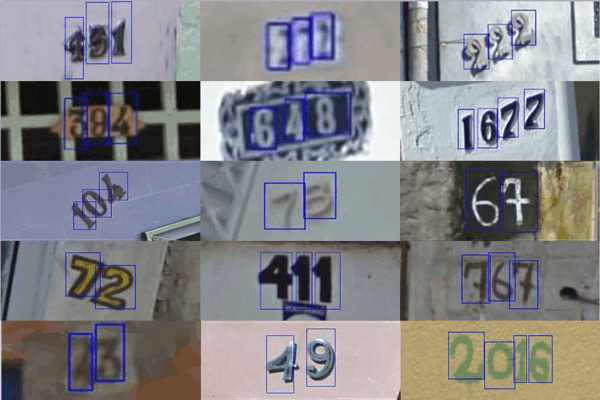
\includegraphics[height=4cm]{googlehousenumbers.jpg}

        \end{column}

        \begin{column}[T]{10cm}
        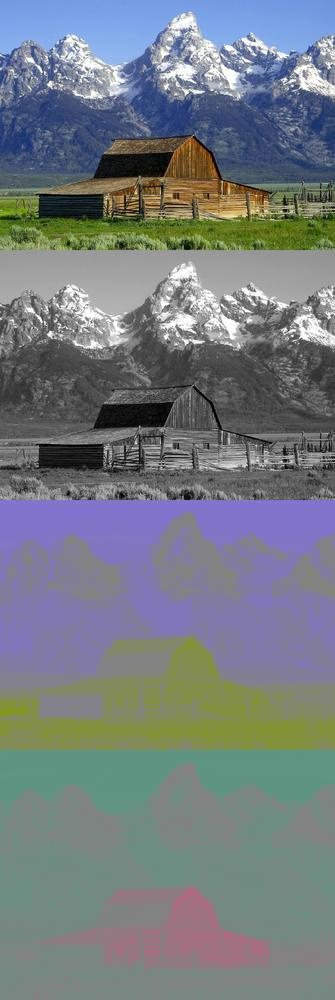
\includegraphics[height=7cm]{YCbCr-separation-small.jpg}
        \end{column}
    \end{columns}
\end{frame} 

\begin{frame}
\frametitle{YCbCr image compression}
    \begin{itemize}
    \item Human eye more sensitive to brightness than color
    \item Can reduce the bandwith of the chrominance channels
    \item Chroma subsampling
    \item NTSC, PAL, MPEG, JPEG
    \item Color quantization
    \end{itemize}
\end{frame}

\begin{frame}
\frametitle{YCbCr image compression}
    \begin{figure}[htb]
    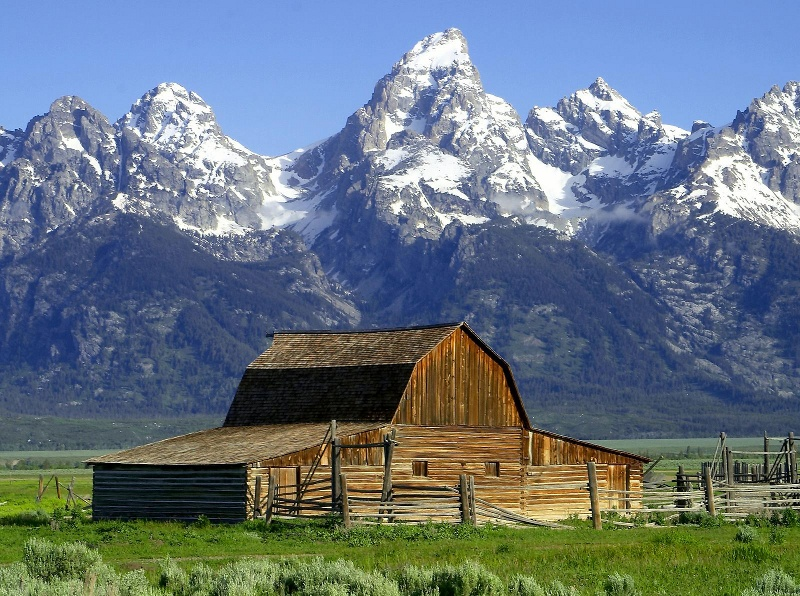
\includegraphics[scale=0.3]{YCbCr-normal.jpg}
    \end{figure}
\end{frame}

\begin{frame}
\frametitle{YCbCr image compression}
    \begin{figure}[htb]
    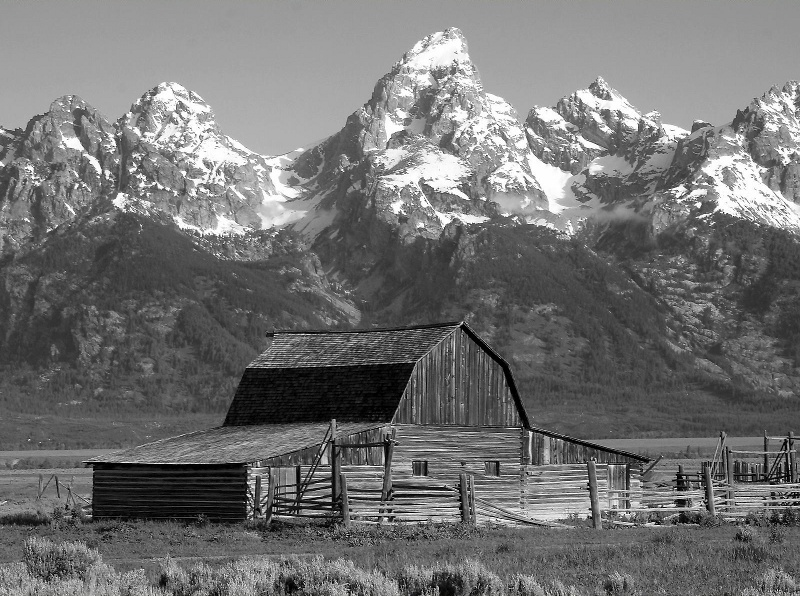
\includegraphics[scale=0.3]{YCbCr-bw.jpg}
    \end{figure}
\end{frame}

\begin{frame}
\frametitle{YCbCr image compression}
    \begin{figure}[htb]
    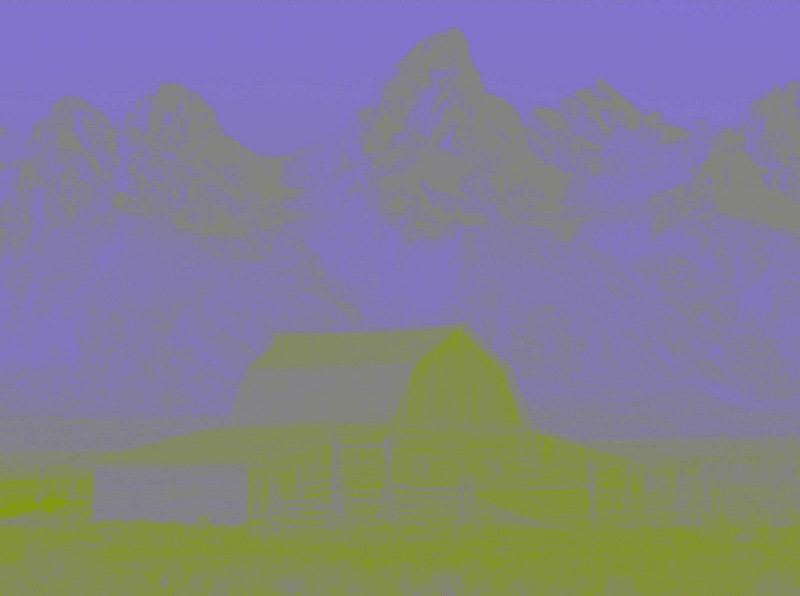
\includegraphics[scale=0.3]{YCbCr-cb.jpg}
    \end{figure}
\end{frame}

\begin{frame}
\frametitle{YCbCr image compression}
    \begin{figure}[htb]
    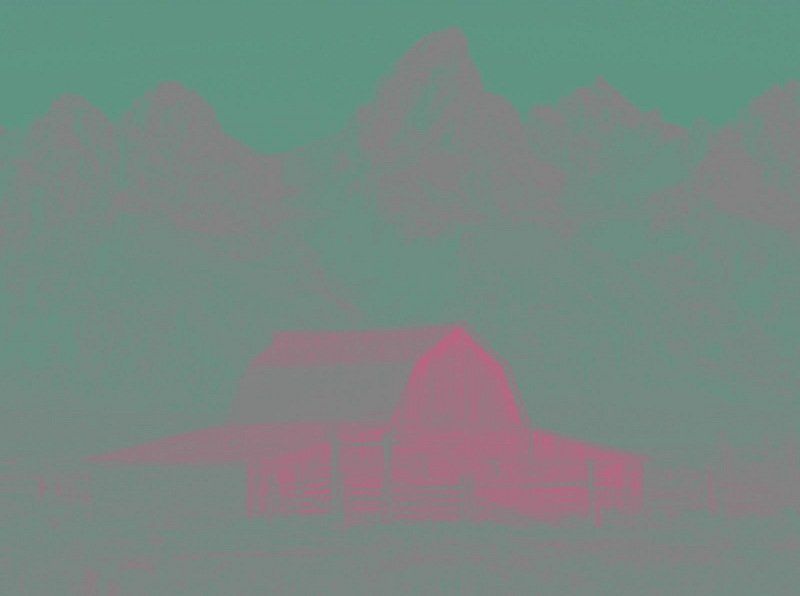
\includegraphics[scale=0.3]{YCbCr-cr.jpg}
    \end{figure}
\end{frame}

\begin{frame}
\frametitle{Podatki}
    \begin{itemize}
    	\item Red-Blue
    		\begin{figure}[]
    			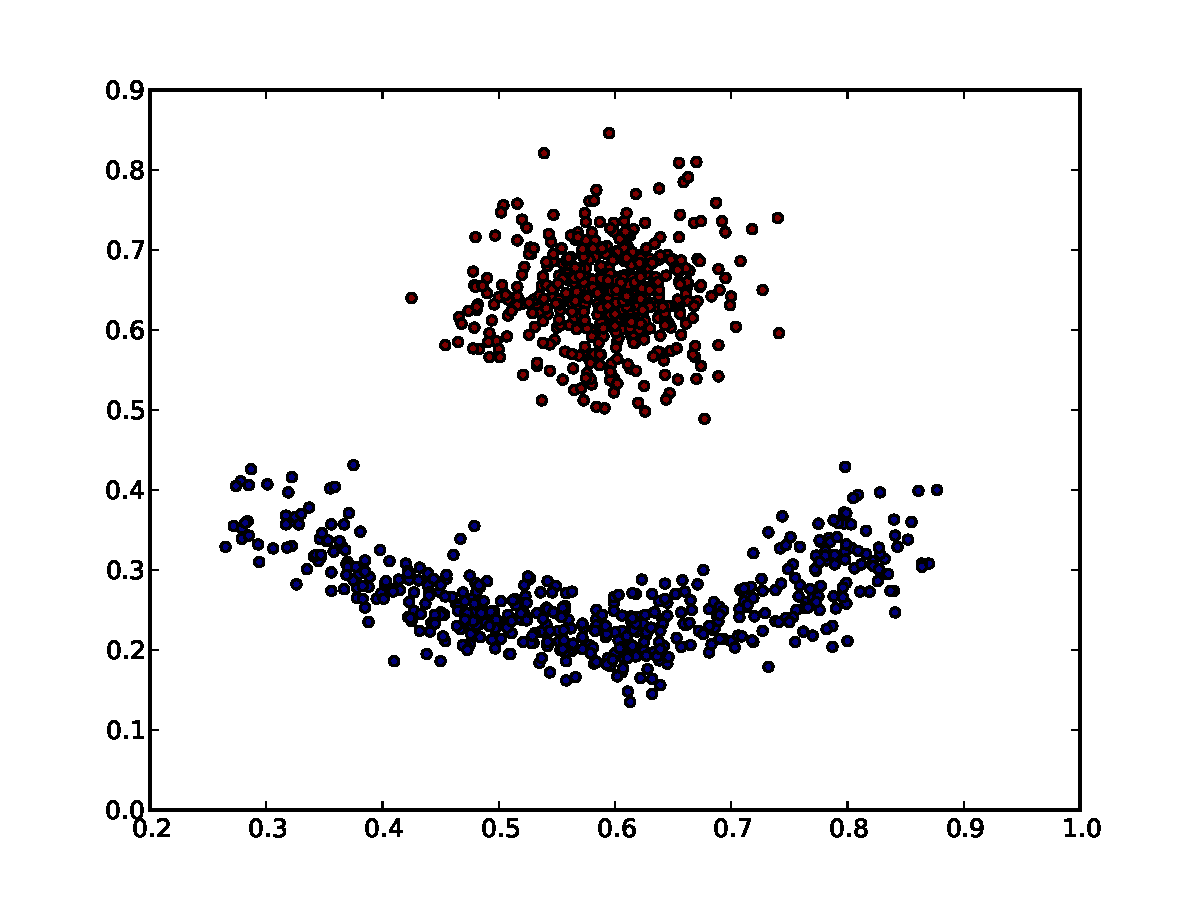
\includegraphics[scale=0.2]{red-blue-clusters.pdf}
    		\end{figure}
   	\item Nested-Circle
    		\begin{figure}[]
    			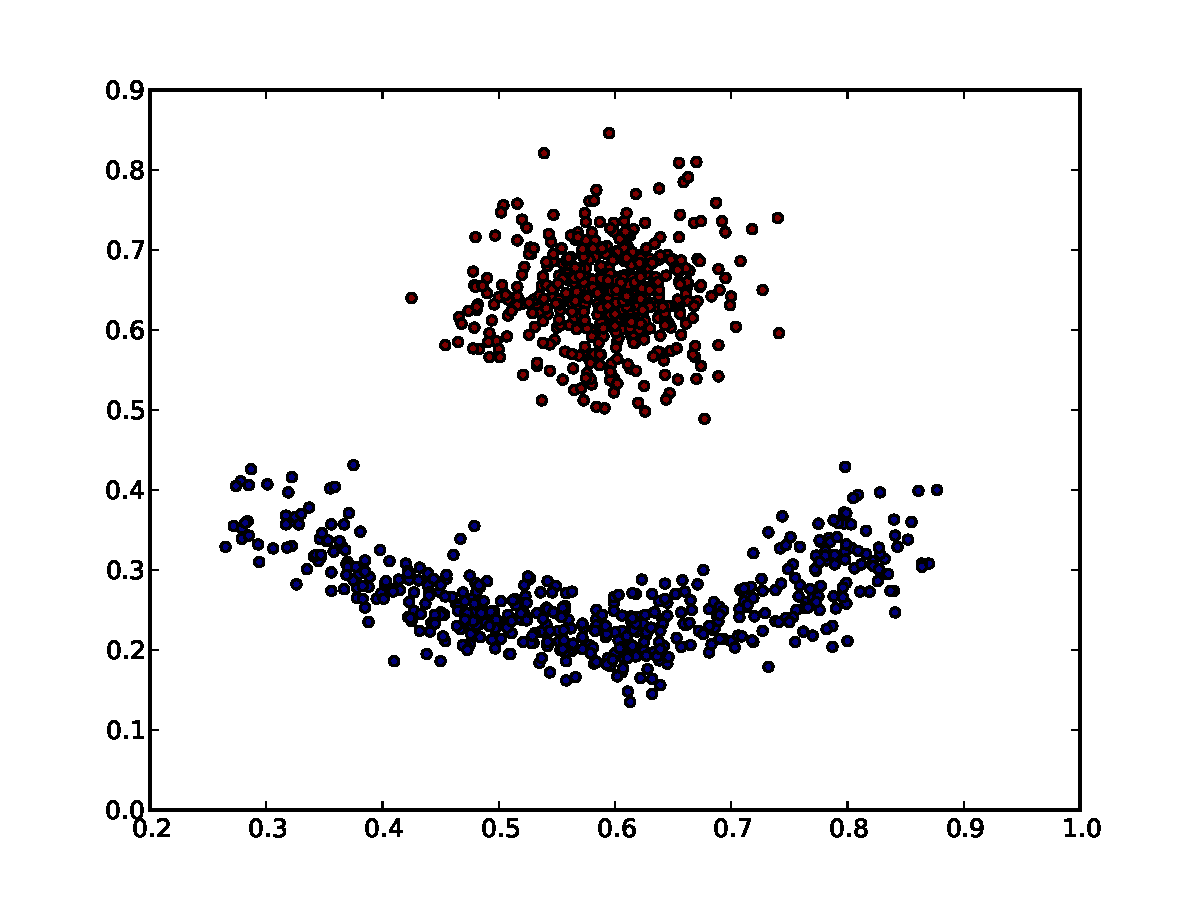
\includegraphics[scale=0.2]{red-blue-clusters.pdf}
    		\end{figure}
    \end{itemize}
\end{frame}

\begin{frame}
\frametitle{Podatki}
    \begin{itemize}
   	\item Half-Moons
    		\begin{figure}[]
    			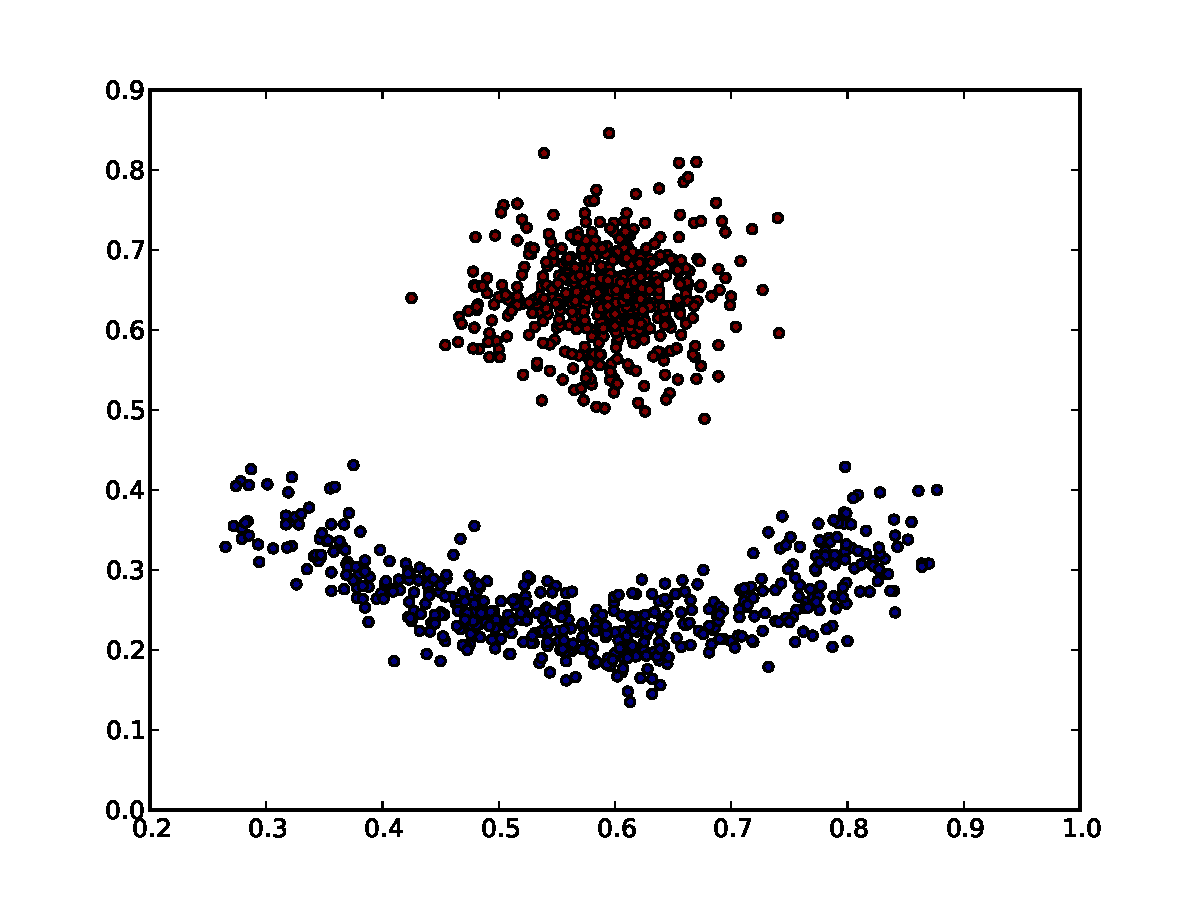
\includegraphics[scale=0.2]{red-blue-clusters.pdf}
    		\end{figure}
    \end{itemize}
\end{frame}

\begin{frame}
\frametitle{Algoritmi}
    \begin{itemize}
    	\item ECMC - Evolving Clustering Method with Constrained minimization
   	\item EM GMM - Expectation Maximization Gaussian Mixture Model
   	\item Spectral clustering
   	\item k-means 
   	\item DBSCAN - Density-Based Spatial Clustering of Applications with Noise
    \end{itemize}
\end{frame}

\begin{frame}
\frametitle{ECMC}
    \begin{itemize}
    	\item Razširitev ECM
   	\item Za vsakega člana grozda velja, da je od centra grozda oddaljen manj kot $D_thr$
   	\item Razširitev spreminja članstvo tako, da član pripada najbližjemu grozdu
    \end{itemize}
\end{frame}

\begin{frame}
\frametitle{ECMC}
    \begin{figure}[]
    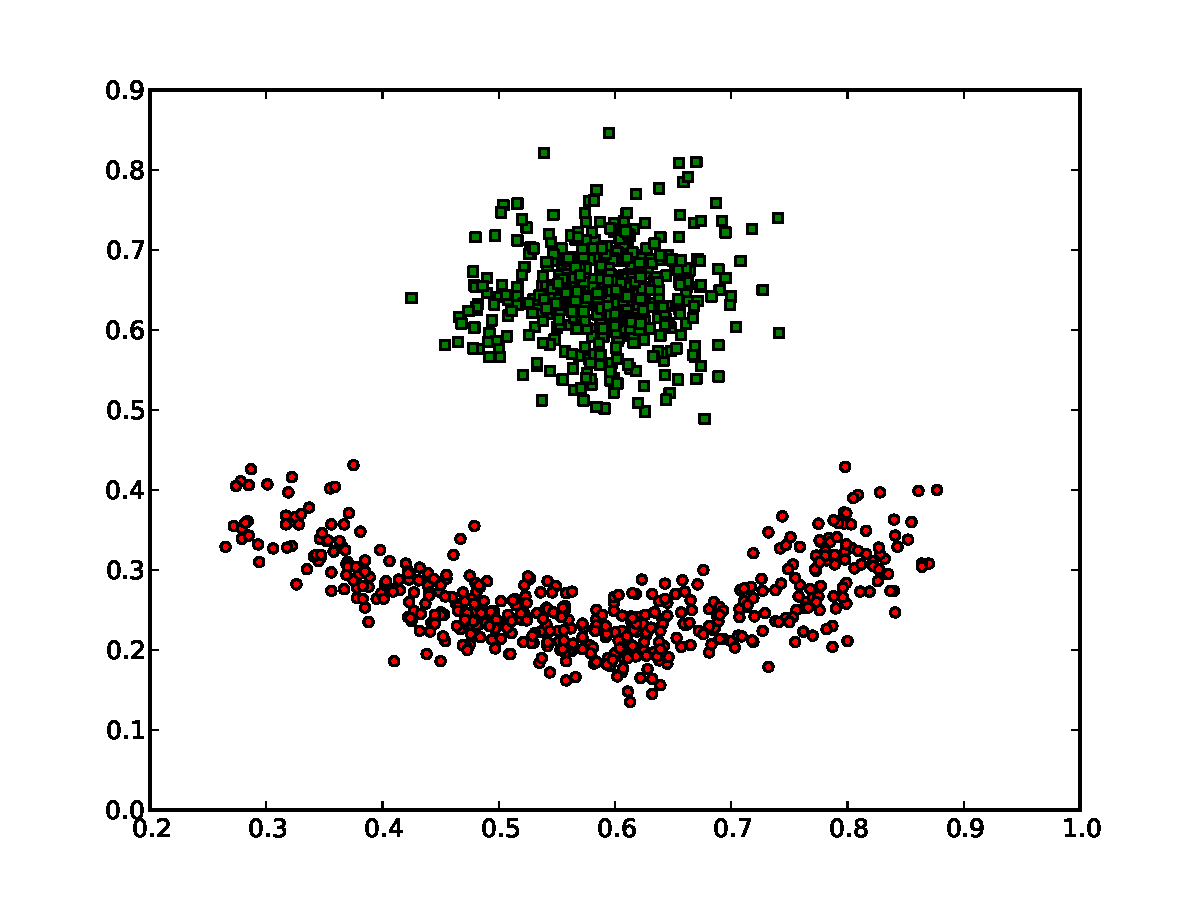
\includegraphics[scale=0.3]{ECMC_red-blue-clusters.pdf}
    \end{figure}
\end{frame}

\begin{frame}
\frametitle{ECMC}
    \begin{figure}[]
    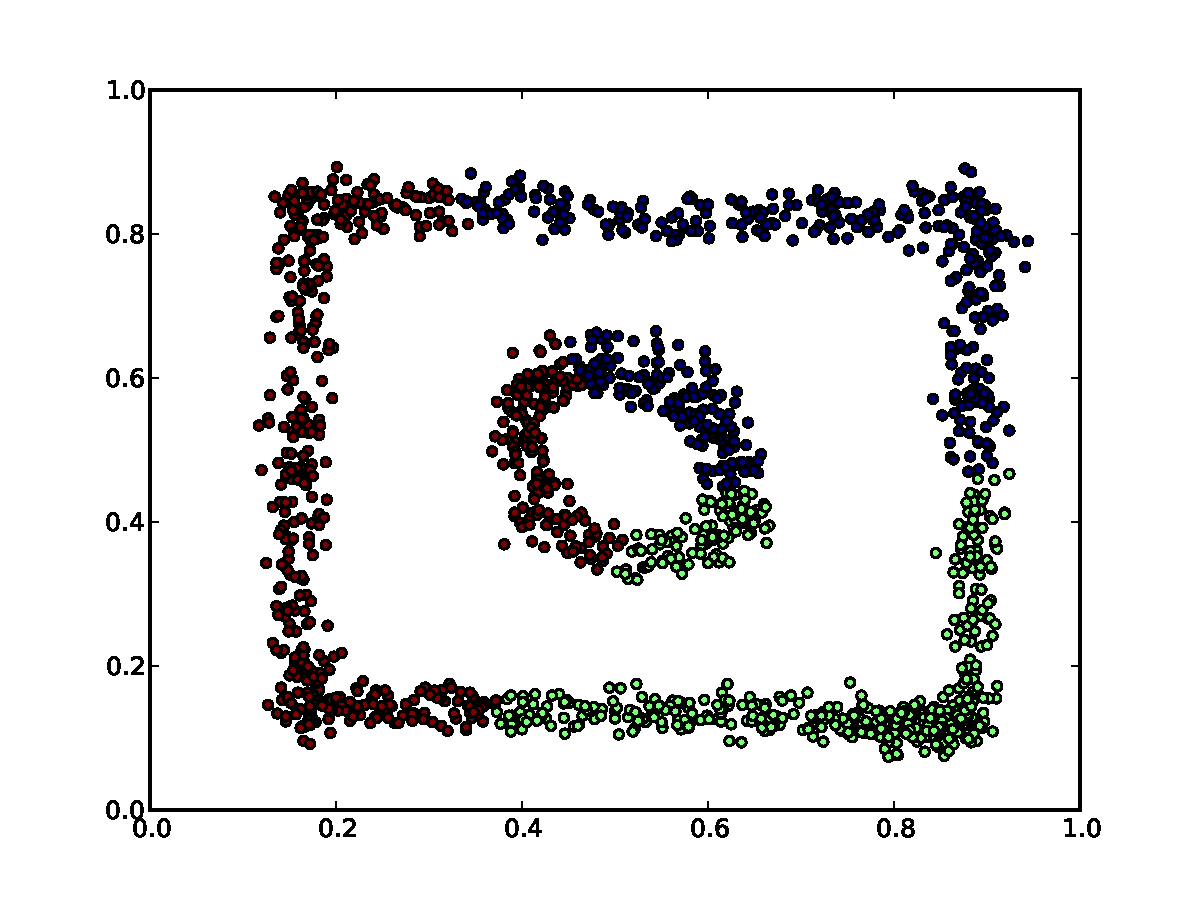
\includegraphics[scale=0.3]{ECMC_circle-weird.pdf}
    \end{figure}
\end{frame}

\begin{frame}
\frametitle{ECMC}
    \begin{figure}[]
    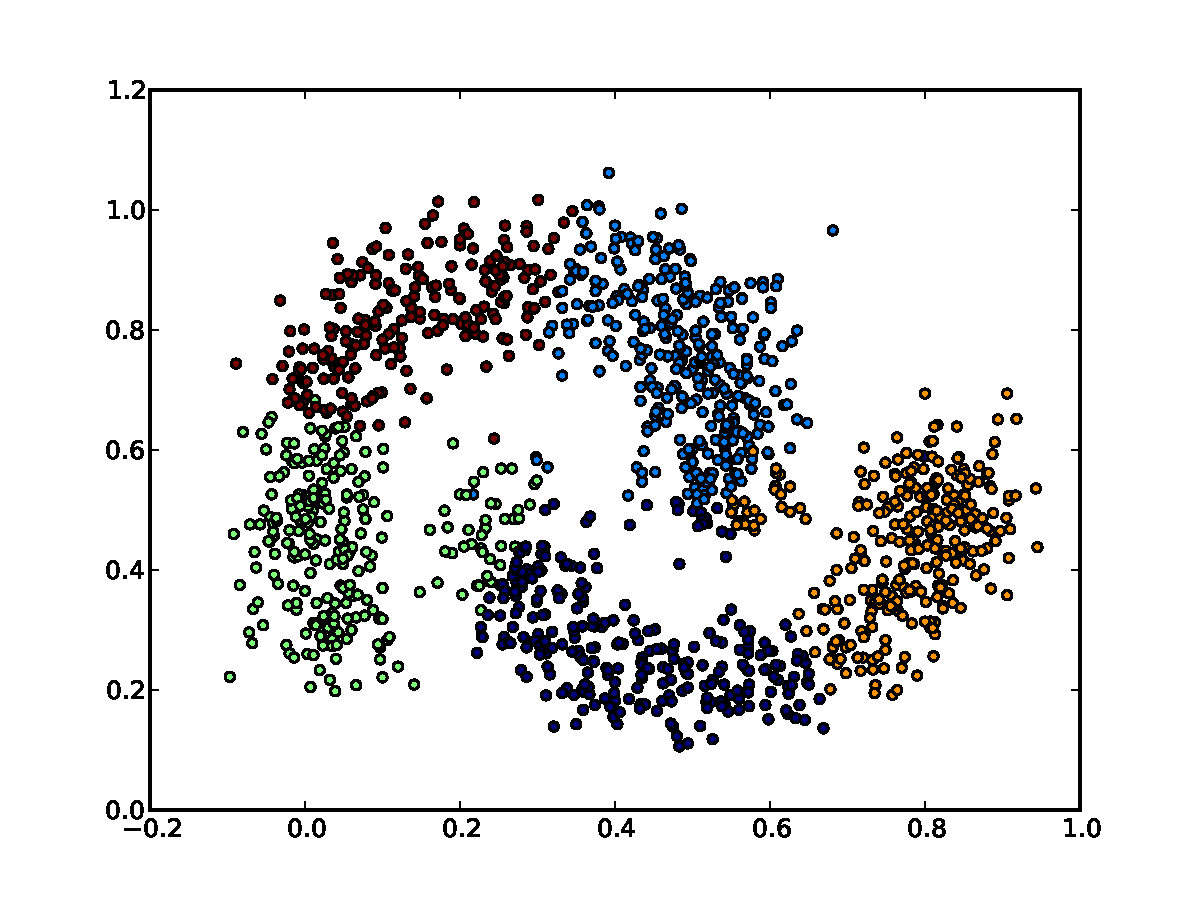
\includegraphics[scale=0.3]{ECMC_half-moons.pdf}
    \end{figure}
\end{frame}

\end{document}
